\subsection{Embarrassing parallelism}
Some problems are inherently parallel, containing no dependencies between subtasks. They can be dissected into a set of distinct work-units that can be executed concurrently.
Such tasks are referred to as ``embarrassingly parallel''.

Many \emph{functional programming} primitives, such as \emph{Map}, are embarrassingly parallel, or parallelisable at some level of granularity.
When transforming a dataset, any operation where the resultant state of each element in the output only depends on a single input can be easily scheduled across many compute units.

\begin{figure}[h]
  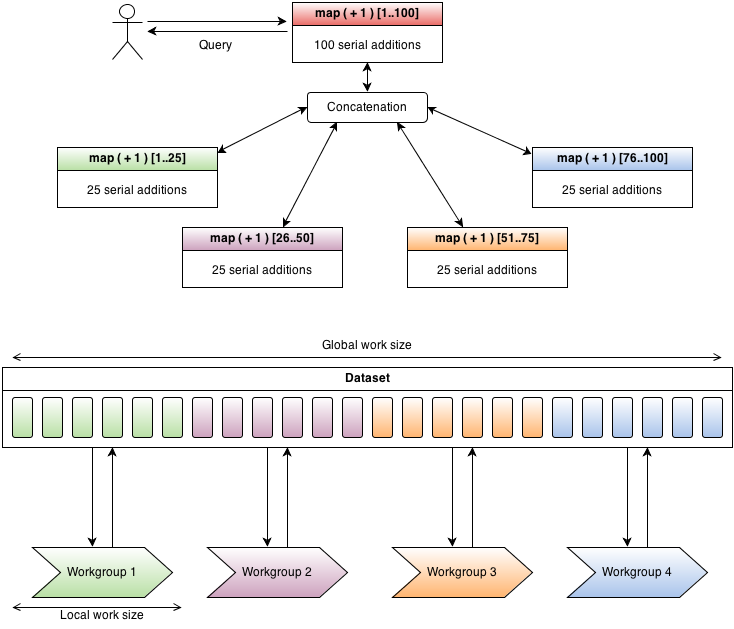
\includegraphics[width=0.8\textwidth]{./figures/map_task.png}
  \caption{A partitioning of \emph{map} computation over several compute devices.}
  \label{fig:map_task}
\end{figure}

Other tasks are more complicated, and require structuring as the composition of concurrent subtasks.
In the worst case, computing a result requires communication and synchronisation between parallel subproblems.

When manually parallelising code, programmers must be familiar with designing multithreaded algorithms. Subcomponents that cooperate must be produced in order to achieve processing speed-up.

This effort is often unnecessary. Certain primitives are known to be suitable for parallel execution. These can be algorithmically scheduled across multiple compute units. By automating this translation and scheduling task, programmers can achieve increased throughput without the need for extensive studying and configuration.

